
\chapter{The Poisson-Boltzmann Analytical Method}



\section{PB-AM formulation}

PB-AM is an analytical solution to the linearized Poisson-Boltzmann equations for multiple spherical objects of arbitrary charge distribution in an ionic solution.  The linearized Poisson-Boltzmann equation is given as:

\[ \nabla [\epsilon(r) \nabla\phi(r)] - \epsilon(r) \kappa^2\phi(r) = 4 \pi \rho(r) \] %∇[ϵ(r)∇Φ(r)]-ϵ(r) κ^2 Φ(r)=4πρ(r)

\[ \phi_{out}^{(i)}= \phi_{out}^{(i)} \biggr |_{r=a_i } \]

\[\epsilon_s \frac{\partial \phi_{out}^{(i)}}{\partial r} =   \epsilon_s \frac{\partial \phi_{out}^{(i)}}{\partial r} \biggr |_{r=a_i } \]

Exploiting fast-multipole methods, this boundary value problem can be reduced to the following system of linear equations.  

\[ A = \Gamma \cdot (\Delta \cdot T \cdot A + E) \]

A(i) represents the effective multipole expansion of the charge distributions of molecule (i). 
E(i) is the free charge distribution of molecule (i). $\Gamma$ is a dielectric boundary-crossing 
operator, $\Delta$ a cavity polarization operator, T an operator that transforms the multipole 
expansion to a local coordinate frame.  More details on the method are available in Lotan, 
Head-Gordon (2006)\footnote{Lotan, I.; Head-Gordon, T. L. . \textit{J. Chem. Theor. Comp.} 2006, 
\textit{2}, 541\---555.}. \\

\subsection{Physical Calculations}

From the above formulation, computation of the interaction energies ($\Omega^{(i)}$) is given as follows:

\[\Omega^{(i)}=\frac{1}{\epsilon_s} \left \langle \sum_{j \ne i}^N  T \cdot A^{(j) } ,  A^{(i) } \right \rangle \]

Where $\langle  M, N \rangle$ denotes the inner product. When energy is computed, forces follow as:

\[ \textbf{F}^{(i)} = \nabla_i \Omega^{(i)}=\frac{1}{\epsilon_s} [ \langle \nabla_i \,T \cdot A^{(i) } ,  A^{(i) } \rangle +  \langle T \cdot A^{(i) } ,   \nabla_i \, A^{(i) } \rangle ]\]


% Additonally, the torque $\tau^{(i)}_j$ on molecule $i$ due to a charge $q^{(i)}_j$ is calculated as follows:
The method to calculate the torque $\boldsymbol{\tau}^{(i)}$ on molecule is outside the scope of this manual, but is discussed extensively in Lotan, Head-Gordon (2006).

\subsection{Brownian Dynamics}

Brownian dynamics simulations are implemented by treating each molecule as a Brownian particle experiencing a conservative force $\textbf{F}^{(i)}$ and torque $\boldsymbol{\tau}^{(i)}$, as well as friction and random force due to the solvent. The translation $\Delta r_i$ and rotation $\Delta \theta_i$ for a time step $\Delta t$ are then given by

\[\Delta r^{(i)} = \frac{D_{i, trans} \Delta t}{k_B T} \textbf{F}^{(i)} + \textbf{S}_i(\Delta t)\]
\[\Delta \theta^{(i)} = \frac{D_{i, rot} \Delta t}{k_B T} \boldsymbol{\tau}^{(i)} + \boldsymbol{\Theta}_i(\Delta t)\]

where $D_{i, trans}$ and $D_{i, rot}$ are the translation and rotational diffusion coefficients for molecule $i$, respectively and $\textbf{S}_i(\Delta t)$ and $\boldsymbol{\Theta}_i(\Delta t)$ are the stochastic components of translation and rotation, respectively, which have the following properties:

\[\langle \textbf{S}_i \rangle=0, \qquad \langle \textbf{S}_i^2 \rangle=2D_{i, trans}\Delta t\]
\[\langle \boldsymbol{\Theta}_i \rangle=0, \qquad \langle \boldsymbol{\Theta}_i^2 \rangle=2D_{i, rot}\Delta t\]

\subsection{Electrostatics}

In a similar manner to the interaction energy calculations in the Physical Calculations section, the electrostatics computes the potential at any point in space exterior to the molecules, \textbf{r}, as the inner product of all the solved effective multipole expansions \(A^{(j)}\) with a local multipole expansion of a single positive charge at position, \textbf{r}.

\[\Phi_{out}(\textbf{r})= \frac{1}{\epsilon_s} \left \langle \sum_{j = 1}^N  T \cdot A^{(j) } , \,  A(\textbf{r})  \right \rangle \]

\clearpage


\section{Use}

\subsection{Installation}

To install this program, first download the source code from the GitHub repository: \\

\hspace{1cm}\texttt{\$ git clone https://github.com/davas301/pb\_solvers.git clone\_dir} \\

Then navigate to the cloned directory \texttt{clone\_dir}. From here, make a \texttt{build} directory, use CMake to create a make file and then make the program.  This is done as follows: \\

\hspace{1cm}\texttt{\$ cd clone\_dir} 

\hspace{1cm}\texttt{\$ mkdir build}

\hspace{1cm}\texttt{\$ cd build}

\hspace{1cm}\texttt{\$ cmake ..} 

\hspace{1cm}\texttt{\$ make pbam} \\

An executable named \texttt{pbam} will now be in \texttt{clone\_dir/build/bin}. \clearpage

\section{Program flow}

Here is the general setup of a PB-AM run.

\begin{figure}[!htbp]
  \centering
  \begin{minipage}[b]{0.85\textwidth}
    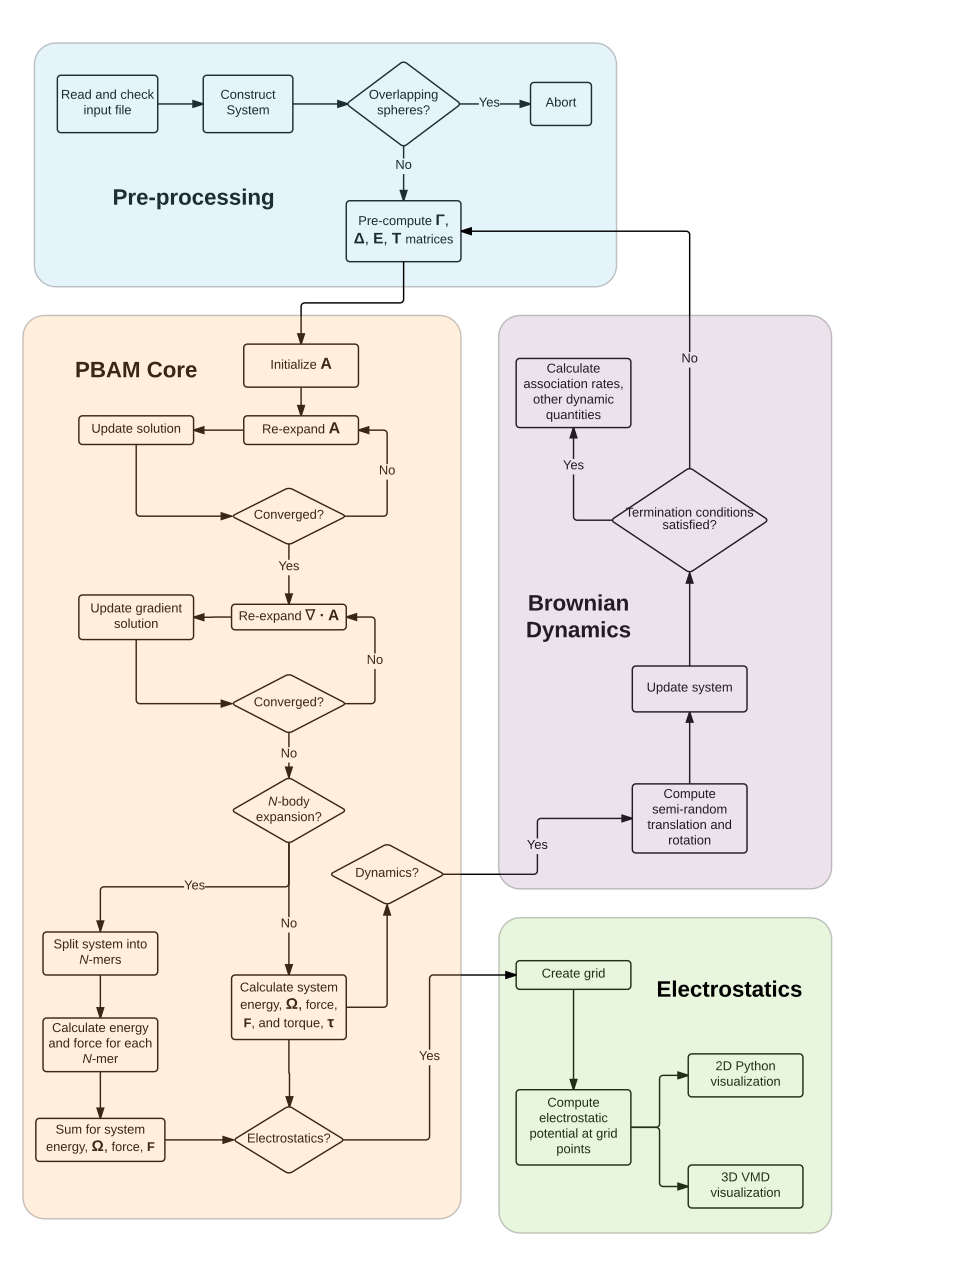
\includegraphics[width=\textwidth]{pbam_flow}
    \caption{Flowchart of PB-AM algorithm.}
    \label{fig:pbsam_cart}
  \end{minipage}
\end{figure}

%%%%%%%%%%%%%%%%%%%%%%%%%%%%%%%%%%%%%%%%%%%%%%%%%%%%%%%%%%%%%%%%%%
%%%%%%%%%%%%%%%%%%%%%%%%%%%%%%%%%%%%%%%%%%%%%%%%%%%%%%%%%%%%%%%%%%
\section{Input Information}

\subsubsection{Input Files}

The program executable requires an input file as a command line parameter. The input file contains the various arguments and parameters that one may wish to set when running the program. Each line of the input file contains a keyword followed by a variable number of whitespace-delimited parameters, e.g.: \\

\texttt{keyword1\qquad param1\qquad param2} \\
\texttt{keyword2\qquad param1\qquad param2\qquad param3} \\

Each keyword is described in the table below, along with its associated parameters.


\newlength{\colthree}
\setlength{\colthree}{10.1cm}
\newlength{\coltwo}
\setlength{\coltwo}{2.9cm}

\begin{tabular}{ c | l | l  }
    \textbf{Keyword} & \textbf{Parameters} & \textbf{Description} \\ \hline
\T runname & \param{name} & \parbox[t]{\colthree}{\param{name} is desired internal name of this run.} \\
\T attypes & \param{numtypes} & \parbox[t]{\colthree}{Set the number of different atom types to \param{numtypes}.}\\
\T pqr & \param{idx} \param{fpath} & \parbox[t]{\colthree}{The molecule index for this xyz file. Provide input PQR file at \param{fpath}.} \\
\T xyz & \param{idx} \param{fpath} & \parbox[t]{\colthree}{The molecule index for this xyz file. Provide input XYZ file at \param{fpath}.} \\
\T transrot & \param{idx} \param{fpath} & \parbox[t]{\colthree}{The molecule type index for this translation/rotation file that can be input instead of a xyz file. Provide input file at \param{fpath}.}\\
\T randorient &  & \parbox[t]{\colthree}{If you want your molecules to be randomly rotated, use this flag} \\
\T units & \param{units} & \parbox[t]{\colthree}{Set the units of output to \param{units}. The current options are: \texttt{jmol} (Joules/mole), \texttt{kT} (kT/e) and \texttt{kcalmol} (kCal/mole).}\\
\T salt & \param{con} & \parbox[t]{\colthree}{Set salt concentration in the system to \param{con}.}\\
\T temp & \param{T} & \parbox[t]{\colthree}{Set system temperature to \param{T}}\\
\T idiel & \param{ival} & \parbox[t]{\colthree}{Set the interior dielectric constant to \param{ival}.} \\
\T sdiel & \param{sval} & \parbox[t]{\colthree}{Set the solvent dielectric constant to \param{sval}.} \\
\T pbc & \param{boxlength} & \parbox[t]{\colthree}{Set size of periodic box to \param{boxlength}.}\\
\T random & \param{seed} & \parbox[t]{\colthree}{Seed the internal random number generator with \param{seed}.} \\
\T type & \parbox[t]{\coltwo}{\param{idx} \param{ct} \param{movetype} \param{dtr} \param{drot}} & \parbox[t]{\colthree}{Set attributes of an atom type, where \param{idx} is the integer id of this type, which can be 1 to \param{numtypes} (above). \param{ct} is the number of atoms of this type in the system and \param{movetype} describes the way this type is allowed to move in a dynamics run (\texttt{move}, \texttt{rot}, or \texttt{stat}). If \param{movetype} is \texttt{move}, then a translational diffusion coefficient \param{dtr} and a rotational diffusional coefficient \param{drot} are required. If \param{movetype} is \texttt{rot} then just \param{drot} is required. \B}\\
\hline
\end{tabular}


\setlength{\colthree}{8.1cm}
\setlength{\coltwo}{2.5cm}

\begin{tabular}{ c | l | l}
    \textbf{Keyword} & \textbf{Parameters} & \textbf{Description} \\ \hline

\T runtype electrostatics & \param{gridpts} & \parbox[t]{\colthree}{Will run electrostatics calculations. \param{gridpts} is an optional integer describing the number of evenly spaced points in each dimension to perform calculations on.\B}\\

\T dx & \param{fname} & \parbox[t]{\colthree}{For electrostatics. Will write the results of electrostatics calculations for every 3D grid point to \param{fname}, in the same output format as APBS dx file.\B} \\

\T 3dmap & \param{fname} & \parbox[t]{\colthree}{For electrostatics. Will write the results of electrostatics calculations for points on the surface of the molecules in the system.\B} \\

\T gridct & \param{ct} & \parbox[t]{\colthree}{For electrostatics. \param{ct} is the number of 2D grids to output.\B} \\

\T grid2d & \parbox[t]{\coltwo}{\param{idx} \param{fname} \param{axis} \param{val} } & \parbox[t]{\colthree}{For electrostatics. Set attributes of a grid output where \param{idx} is the integer id of this grid, which can be 1 to \param{ct} (above). Will write output of calculations for a cross section along \param{axis} (\texttt{x}, \texttt{y}, or \texttt{z}) at \param{value}.\B} \\

\hline
  \end{tabular}
  
  
  \begin{tabular}{ c | l | l}
    \textbf{Keyword} & \textbf{Parameters} & \textbf{Description} \\ \hline
\T runtype dynamics & \parbox[t]{\coltwo}{ \param{outname}  \param{ntraj}} & \parbox[t]{\colthree}{Will perform a brownian dynamics run. A directory where trajectory information will be stored in and the number of trajectories is required.\B}  \\

\T termct & \param{ct} & \parbox[t]{\colthree}{Set number of termination conditions to \param{ct}.}  \\

\T termcombine & \param{andor} & \parbox[t]{\colthree}{Set how termination conditions will be combined. \param{andor} should be \texttt{and} or \texttt{or}. Default is \texttt{or}.} \\

\T term & \parbox[t]{\coltwo}{\param{idx} \param{type} \param{val} \param{mols}} & \parbox[t]{\colthree}{Set attributes of a termination condition where \param{idx} is the integer id of this condition, which can be 1 to \param{ct} (above). \param{type} can be \texttt{time},  \texttt{x<=}, \texttt{y<=}, \texttt{z<=}, or \texttt{r<=} (or the \texttt{>=} equivalents of these), \param{val} is the value where the simulation will terminate and \param{mols} is a whitespace-delimited list of molecular indices that this condition applies to (\texttt{time} requires 0, and all else require 1). \B} \\

\T term \param{idx} contact & \parbox[t]{\coltwo}{\param{confile} \param{pad}} & \parbox[t]{\colthree}{Set attributes of contact termination condition, where \param{idx} is the integer id of this condition, \param{confile} is a path to a file containing the contact information, and \param{pad} specifies a correction for the case when the contact distance cannot be reached due to the spherical assumption of the model. See below for more info. \B} \\

\T xyz & \parbox[t]{\coltwo}{\param{idx} \param{trajidx} \param{fpath} }& \parbox[t]{\colthree}{\param{idx} is the molecule index for this xyz file. Provide input XYZ file at \param{fpath}. For the dynamics run, a starting configuration is needed for each trajectory for all the molecule types, so there should be \param{ntraj} xyz lines for each molecule, the trajectory number denoted by \param{trajidx}. \B} \\
\hline
\T runtype energyforce &  \param{outfilename} & \parbox[t]{\colthree}{Will calculate the interaction energy, the forces and torques for the system input. \param{outfilename} is a filename that you would like the information printed to. If none is entered, the information will be printed to the command line.\B}  \\
\hline
  \end{tabular}

\clearpage

\subsection{System inputs: PQR, XYZ, Translation/Rotation and Contact files }

\subsubsection{PQR File}

All the options above require a \textbf{PQR} file name. A PQR file can be generated from a PDB file using the PDB2PQR program, available as a web server or for download at: \\

http://nbcr-222.ucsd.edu/pdb2pqr\_1.9.0/  \\
http://www.poissonboltzmann.org/docs/pdb2pqr-installation/ \\

It may also be formatted manually. The general format of a PQR file is as follows, and is whitespace-delimited: \\

\texttt{recName  serial  atName  resName  chainID  resNum  X  Y  Z  charge rad }\\

  \begin{tabular}{ c | l  }
    \textbf{Parameter} & \textbf{Description} \\ \hline
\texttt{recName} 	&	A string that should either be ATOM or HETATM. \\
\texttt{serial} 	&	An integer that provides the atom index \\
\texttt{atName} 	&	A string that provides the atom name.\\
\texttt{resName}	&	A string that provides the residue name. \\
\texttt{chainID}	&	An optional string that provides the chain ID of the atom.\\
\texttt{residueNumber}  & An integer that provides the residue index.\\
\texttt{X Y Z}	& Three floats that provide the atomic coordinates.\\
\texttt{charge}	& A float that provides the atomic charge (in electrons). \\
\texttt{Rad}		& A float that provides the atomic radius (in \AA).\\
    \hline
  \end{tabular}

\subsubsection{XYZ File}

The \textbf{XYZ} file simply specifies the desired molecule centers for a given molecule type. \\

\texttt{mol1X  mol1Y  mol1Z }\\
\texttt{mol2X  mol2Y  mol2Z }\\
\texttt{mol3X  mol3Y  mol3Z }\\

\subsubsection{Translation/Rotation File}

\textbf{Translation/Rotation} Instead of a XYZ file, one can input a file specifying the translations and rotations that should be applied to 
each molecule of a particular type. For these files, we follow the PDB standard for rotation matrices and translation vectors, 
which is as follows: \\

\texttt{mol1 rot\_1\_11 rot\_1\_12 rot\_1\_13 trans\_1\_1} \\
\texttt{mol1 rot\_1\_21 rot\_1\_22 rot\_1\_23 trans\_1\_2} \\
\texttt{mol1 rot\_1\_31 rot\_1\_32 rot\_1\_33 trans\_1\_3} \\
\texttt{mol2 rot\_2\_11 rot\_2\_12 rot\_2\_13 trans\_2\_1} \\
\texttt{mol2 rot\_2\_21 rot\_2\_22 rot\_2\_23 trans\_2\_2} \\
\texttt{mol2 rot\_2\_31 rot\_2\_32 rot\_2\_33 trans\_2\_3} \\

where \texttt{mol1} and \texttt{mol2} are indices of the molecule of the type this file applies to, \texttt{rot\_i\_jk} is the \texttt{j,k} index
of the rotation matrix for molecule \texttt{i} and \texttt{trans\_i\_j} is the \texttt{j}th element in the translation vector for molecule \texttt{i}.

\subsubsection{Contact File}
\textbf{Contact} files describe contacts between two molecular types. Generally this information is used to determine if a dynamics 
simulation should be terminated (e.g. terminate a simulation after two proteins have docked). The contact file contains lines with the format: \\

\texttt{moltype1  at1 moltype2 at2 dist}\\

where \texttt{moltype1} and \texttt{moltype2} are indices of the molecular types, \texttt{at1} is the index of an atom from the first 
molecular type, \texttt{at2} is the index of an atom from the second molecular type and \texttt{dist} is the maximum distance between
the two atoms that defines the contact.  Note that sometimes these distances cannot be reached due to the assumption in this model that 
the molecule is spherical. To correct for this case, one must specify a "pad"  distance that is defined as the maximum distance between 
the radial projections of the atoms onto the surface of their respective spheres that defines a contact.

\clearpage



%%%%%%%%%%%%%%%%%%%%%%%%%%%%%%%%%%%%%%%%%%%%%%%%%%%%%%%%%%%%%%%%%%
%%%%%%%%%%%%%%%%%%%%%%%%%%%%%%%%%%%%%%%%%%%%%%%%%%%%%%%%%%%%%%%%%%

\section{Example files and outputs}

\subsection{Physical calculations}

\textbf{Example physical calculations runfile} \\

name:  \texttt{run.energyforce.inp}:
\begin{lstlisting}[style = MyBash]
runtype energyforce
runname energyforce.2sp.jmol.out

units jmol
salt 0.01
temp 353
idiel 4 
sdiel 78

attypes 1
type 1 2
pqr 1 single_charge.pqr
xyz 1 positions_2.xyz
\end{lstlisting}
\medskip

The files for PQR and XYZ are: 

name:  \texttt{single\_charge.pqr}:
\begin{lstlisting}[style = MyBash]
ATOM      1  N   NTR     0       1.000   0.000   0.000 -1.0000 3.7300
ATOM      1  N   NTR     0       0.000   1.000   0.000 -1.0000 6.3200
\end{lstlisting}

\medskip

name:  \texttt{positions\_2.xyz}:
\begin{lstlisting}[style = MyBash]
-10.0  23.4  -8.7
  0.0   0.0  -2.5
\end{lstlisting}
\medskip

To run: 
\begin{lstlisting}[style = MyBash]
$$ ../../bin/pbam run.energyforce.inp
\end{lstlisting}
\medskip

And the resulting file: 

name: \texttt{energyforce.2sp.jmol.out}:
\begin{lstlisting}[style = MyBash]
My units are Joules/Mol
MOLECULE #1
        POSITION: [-10, 23.4, -8.7]
        ENERGY: 1328.86
        FORCE: 1.19858e+08, [-36.6012 1.19858e+08 -1.65408e-05]
        TORQUE: 1.78426e+06, [1.28425 1.78426e+06 1.9978e-06]
MOLECULE #2
        POSITION: [0, 0, -2.5]
        ENERGY: 1328.86
        FORCE: 1.19858e+08, [36.6012 -1.19858e+08 1.65408e-05]
        TORQUE: 1.78354e+06, [1.28372 1.78354e+06 1.99699e-06]
\end{lstlisting}


\subsection{Brownian Dynamics}

\textbf{Example dynamics runfile} \\

name:  \texttt{run.dynamics.inp}:
\begin{lstlisting}[style = MyBash]
runtype dynamics 2
runname dyn_cont_barn

salt 0.01
temp 298
idiel 4 
sdiel 78

termct 1
termcombine or
term 1 contact 2.5 1 2

attypes 2
type 1 2 move 0.015 0.000045
pqr 1 1BRS_chainA.pqr
xyz 1 1 pos_1_1.xyz
xyz 1 2 pos_1_2.xyz

type 2 2 move 0.015 0.000045
pqr 2 1BRS_chainD.pqr
xyz 2 1 pos_2_1.xyz
xyz 2 2 pos_2_2.xyz
\end{lstlisting}
\medskip

The files for PQR (first 5 lines) and XYZ files for the first trajectories are: 

name:  \texttt{1BRS\_chainA.pqr}:
\begin{lstlisting}[style = MyBash]
ATOM   1700  N    ALA B   1      20.757 52.394 30.692     0.1414  1.8240
ATOM   1702  CA   ALA B   1      20.602 52.680 29.268     0.0962  1.9080
ATOM   1703  C    ALA B   1      19.286 52.138 28.675     0.6163  1.9080
ATOM   1704  O    ALA B   1      18.578 51.351 29.318    -0.5722  1.6612
ATOM   1705  CB   ALA B   1      21.739 52.033 28.476    -0.0597  1.9080
\end{lstlisting}

\medskip

name:  \texttt{pos\_1\_1.xyz}:
\begin{lstlisting}[style = MyBash]
61.25 61.25 61.25
-26.25 61.25 -26.25
\end{lstlisting}
\medskip

name:  \texttt{1BRS\_chainD.pqr}:
\begin{lstlisting}[style = MyBash]
ATOM      1  N    LYS D   1      48.330 40.393  9.798     0.0966  1.8240
ATOM      2  CA   LYS D   1      47.401 39.287  9.370    -0.0015  1.9080
ATOM      3  C    LYS D   1      47.507 38.911  7.890     0.7214  1.9080
ATOM      4  O    LYS D   1      47.126 39.582  6.905    -0.6013  1.6612
ATOM      5  CB   LYS D   1      45.995 39.632  9.817     0.0212  1.9080
\end{lstlisting}

\medskip

name:  \texttt{pos\_2\_1.xyz}:
\begin{lstlisting}[style = MyBash]
-26.25 61.25 61.25
61.25 -26.25 61.25
\end{lstlisting}
\medskip

To run: 
\begin{lstlisting}[style = MyBash]
$$ ../../bin/pbam run.dynamics.inp
\end{lstlisting}
\medskip

And the resulting files: 

name: \texttt{dyn\_cont\_barn\_[traj\#].xyz}: VMD readable XYZ file that shows the trajectory of molecules in the system. The time that is snapshot was printed from is given on the same line as the word Atom. The atoms of your input file are currently labeled N, and the coarse-grain center is labeled "X" in the first column of the XYZ file.

\begin{lstlisting}[style = MyBash]
3135
Atoms. Timestep (ps): 0
N   -7.241   -0.530   18.703
N   -6.015   -0.503   17.910
N   -5.784    0.840   17.188
N   -6.682    1.690   17.128
N   -6.066   -1.580   16.827
N   -7.519   -1.481   18.863
N   -7.084   -0.079   19.584
\end{lstlisting}
\medskip

name: \texttt{dyn\_cont\_barn\_[traj\#].dat}: Statistics from simulation printed out at the same time as each XYZ snapshot. The energy is not computed and should be ignored.

\begin{lstlisting}[style = MyBash]
My units are Internal. Time (ps) 500.4
MOLECULE #1
	POSITION: [0, 0, 0]
	ENERGY: 0
	FORCE: 3.39124e-06, [1.69863e-06 2.07547e-06 6.5356e-07]
	TORQUE: 2.55224e-05, [-2.11728e-05 1.00774e-05 3.08631e-05]
MOLECULE #2
	POSITION: [87.211, 43.861, 21.691]
	ENERGY: 0
	FORCE: 3.65373e-06, [-1.87502e-06 -2.21744e-06 -7.27314e-07]
	TORQUE: 1.91656e-05, [8.14396e-06 -1.22678e-05 1.56284e-05]
\end{lstlisting}
\medskip

name: \texttt{dyn\_nam\_barn.stat }: Details about how each simulation has terminated and the time at which this occurred.
\begin{lstlisting}[style = MyBash]
Molecule type 1 has fulfilled condition: r >= 500.00;	 at time (ps) 1.32367e+06
Molecule type 1 has fulfilled condition: r >= 500.00;	 at time (ps) 1.15712e+06
System has fulfilled condition: Type 0 and Type 1 are within  2.50;	 at time (ps) 1.90603e+06
Molecule type 1 has fulfilled condition: r >= 500.00;	 at time (ps) 2.18533e+06
System has fulfilled condition: Type 0 and Type 1 are within  2.50;	 at time (ps) 1.59066e+06
\end{lstlisting}


\subsection{Electrostatics}

\textbf{Example electrostatics runfile} \\

name:  \texttt{run.electrostatic.inp}:
\begin{lstlisting}[style = MyBash]
runtype electrostatics 140
runname electrostatic

units kT
salt 0.01
temp 298
idiel 4 
sdiel 78

dx out.dx

3dmap electro_map.out

gridct 2
grid2D 1 out.x.0.dat x 0
grid2D 2 out.x.-1.dat x -1

attypes 2
type 1 2
pqr 1 single_charge.pqr
xyz 1 positions_2.xyz

type 2 2
pqr 2 pos_charge.pqr
xyz 2 positions_pos.xyz
\end{lstlisting}
\medskip

The files for PQR and XYZ files are: 

name:  \texttt{single\_charge.pqr}:
\begin{lstlisting}[style = MyBash]
ATOM      1  N   NTR     0       0.000   1.000   0.000  4.0000 0.3200
ATOM      1  N   NTR     0       0.000   0.000  -1.000  4.0000 0.3200
ATOM      1  X   CEN     0       0.000   0.000   0.000  0.0000 2.0000
\end{lstlisting}

\medskip

name:  \texttt{positions\_2.xyz}:
\begin{lstlisting}[style = MyBash]
  0.0   0.0  -5.0
  0.0   0.0   5.0
\end{lstlisting}
\medskip

name:  \texttt{pos\_charge.pqr}:
\begin{lstlisting}[style = MyBash]
ATOM      1  N   NTR     0       0.000   1.000   0.000 -4.0000 0.3200
ATOM      1  N   NTR     0       0.000   0.000  -1.000 -4.0000 0.3200
ATOM      1  X   CEN     0       0.000   0.000   0.000  0.0000 2.0000
\end{lstlisting}

\medskip

name:  \texttt{positions\_pos.xyz}:
\begin{lstlisting}[style = MyBash]
  0.0   5.0   0.0
  0.0  -5.0   0.0
\end{lstlisting}
\medskip

To run: 
\begin{lstlisting}[style = MyBash]
$$ ../../bin/pbam run.electrostatic.inp
\end{lstlisting}
\medskip

And the resulting files: 

name: \texttt{out.dx}:
\begin{lstlisting}[style = MyBash]
# Data from PBAM Electrostat run
# My runname is out.dx and units kT/e
object 1 class gridpositions counts 140 140 140
origin -4 -9 -9
delta 0.0571429 0.0e+00 0.0e+00
delta 0.0e00 0.128571 0.0e+00
delta 0.0e00 0.0e+00 0.128571
object 2 class gridconnections counts 140 140 140
object 3 class array type double rank 0 items 2744000 data follows
2.7203115e-01  3.0271755e-01  3.3459723e-01  
3.6769040e-01  4.0201595e-01  4.3759129e-01 
.....
-1.3185519e-01  -1.5849252e-01  -1.8359631e-01
-2.0722087e-01  -2.2942006e-01  -2.5024714e-01
-2.6975467e-01  -2.8799442e-01
attribute "dep" string "positions"
object "regular positions regular connections" class field
component "positions" value 1
component "connections" value 2
component "data" value 3
\end{lstlisting}
\medskip

name: \texttt{electro\_map.out}:
\begin{lstlisting}[style = MyBash]
# Data from PBAM Electrostat run
# My runname is electro_map.out and units kT/e
grid 10 10 10
origin -4 -9 -9
delta 0.8 1.8 1.8
  0.00825   0.00006  -2.90002 -5.899956 
  0.00822   0.00071  -2.90002 -5.902602 
\end{lstlisting}
\medskip

name: \texttt{out.x.0.dat}:
\begin{lstlisting}[style = MyBash]
# Data from PBAM Electrostat run
# My runname is out.x.0.dat
units kT
grid 140 140 
axis x 0 
origin -9 -9
delta 0.128571 0.128571
maxmin 39.23 -39.23
   0.3605004     0.4030045     0.4474874     0.4940082     0.5426260     0.5933995
\end{lstlisting}




